% !TeX spellcheck = fr_FR

% TODO: Replace scan images with clean text where possible

\documentclass[a4paper, 10pt]{report}

\usepackage[french]{babel}
\usepackage[T1]{fontenc}

\usepackage{amsmath, amssymb, amsfonts}

\usepackage{hyperref}
\usepackage{geometry}

\usepackage{xcolor}
\usepackage{graphicx}

\usepackage{fancyhdr}
\usepackage{lastpage}

\usepackage{enumitem}

\geometry{
	a4paper,
	left=25mm,
	right=25mm,
	top=35mm,
	bottom=25mm,
	headsep=5mm,
	headheight=20mm,
}

\definecolor{solution}{HTML}{E5E4E2}
\providecommand{\abs}[1]{\lvert#1\rvert}
\providecommand{\norm}[1]{\lVert#1\rVert}

\begin{document}
	
	\renewcommand{\headrule}{%
		\vspace{-4pt}\hrulefill
		\raisebox{-6.8pt}{\ 
\includegraphics[height=5mm]{../../icon.png}}
		\hrulefill
	}	
	\pagestyle{fancy}
	\fancyhf{}
	
	\fancyhead[L]{\small \slshape Automne 2024}
	\fancyhead[C]{\Large \bfseries Analyse I - Série 02}
	\fancyhead[R]{\small Buff Mathias}
	\fancyfoot[L]{
		\small Source files available at:
		\href{https://github.com/MathiasBuff/bsc-math}
		{github.com/MathiasBuff/bsc-math}
	}
	\fancyfoot[R]{
		\small Page \thepage
		\hspace{1pt} /
		\pageref*{LastPage}
	}
	
	\noindent
	\textbf{Exercice 1.} Écrire la négation des assertions suivantes.
	
	\begin{enumerate}[label=(\roman*)]
		\item $\exists x \in \mathbb{R},
			\exists \delta > 0,
			\forall y \in \mathbb{R},
			[\abs{x - y} \leq \delta \implies f(x) \geq f(y)]$\\
		(où $f$ est une fonction de $\mathbb{R}$ dans $\mathbb{R}$)
		%
		\item $\forall x \in \mathbb{R},
		\forall \epsilon > 0,
		\exists \delta > 0,
		\forall y \in \mathbb{R},
		[\abs{x - y} < \delta \implies \abs{f(x) - f(y)} \leq \epsilon]$\\
		(où $f$ est une fonction de $\mathbb{R}$ dans $\mathbb{R}$)
		%
		\item $\forall \epsilon > 0,
			\exists N \in \mathbb{N},
			\forall x \in \mathbb{R},
			\forall n \geq N,
			[n \geq N \implies \abs{f_n(x) - f(x)} \leq \epsilon]$\\
		(où $f$ est une fonction de $\mathbb{R}$ dans $\mathbb{R}$)
		%
		\item $\forall E \subset \mathbb{N},
			[E \neq \emptyset \implies (\exists n \in E,
				\forall m \in E, m \geq n)]$
		%
		\item $\forall E \subset \mathbb{R},
			[E \neq \emptyset \implies \exists a \in \mathbb{R},
				((\forall b \in E : b \leq a)\
				\text{et}\
				(\forall \epsilon > 0,
					\exists b \in E : b \geq a - \epsilon))]$
	\end{enumerate}
	
	\colorbox{solution}
	{
		\begin{minipage}{0.9\textwidth}
			\begin{enumerate}[label=(\roman*)]
				\item $\forall x \in \mathbb{R},
				\forall \delta > 0,
				\exists y \in \mathbb{R},
				[\abs{x - y} \leq \delta \ \text{et}\ f(x) < f(y)]$
				%
				\item $\exists x \in \mathbb{R},
				\exists \epsilon > 0,
				\forall \delta > 0,
				\exists y \in \mathbb{R},
				[\abs{x - y} < \delta \ \text{et}\ \abs{f(x) - f(y)} > \epsilon]$
				%
				\item $\exists \epsilon > 0,
				\forall N \in \mathbb{N},
				\exists x \in \mathbb{R},
				\exists n \geq N,
				[n \geq N \ \text{et}\ \abs{f_n(x) - f(x)} > \epsilon]$
				%
				\item $\exists E \subset \mathbb{N},
				[E \neq \emptyset \ \text{et}\ (\forall n \in E,
				\exists m \in E, m < n)]$
				%
				\item $\exists E \subset \mathbb{R},
				[E \neq \emptyset \ \text{et}\ \forall a \in \mathbb{R},
				((\exists b \in E : b > a)\
				\text{ou}\
				(\exists \epsilon > 0,
				\forall b \in E : b < a - \epsilon))]$
			\end{enumerate}
		\end{minipage}
	}
	
	\vspace{5mm}
	\noindent
	\textbf{Exercice 2.} (Différence symétrique). L'opération
	$\bigtriangleup$ est définie sur les ensembles $A, B \subset E$
	par $A \bigtriangleup B = (A \cap B^C) \cup (B \cap A^C)$.
	
	\begin{enumerate}[label=(\roman*)]
		\item Montrer que $A \bigtriangleup B =
			(A \cup B) \setminus (A \cap B)$
		%
		\item Vérifier que $(A \bigtriangleup B = \emptyset)
			\iff (A = B)$
	\end{enumerate}
	
	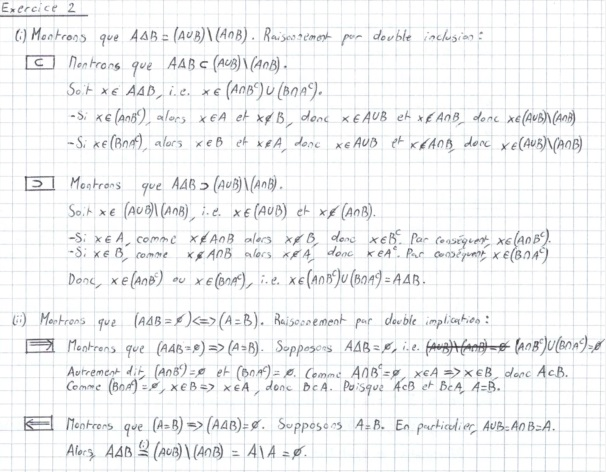
\includegraphics{ex02.jpg}
	
	\newpage
	
	\fancyhf{}
	\renewcommand{\headrule}
	{\rule{\textwidth}{0pt}}
	\fancyfoot[R]{
		\small Page \thepage
		\hspace{1pt} /
		\pageref*{LastPage}
	}
	
	\noindent
	\textbf{Exercice 3.} Expliquer verbalement ce que signifient les
	assertions suivantes et écrire leur négation.
	
	\begin{enumerate}[label=(\roman*)]
		\item $\forall n \geq 0, u_n < u_{n+1}$
		(où $(u_n)$ est une suite réelle)
		%
		\item Soit $f : E \to \mathbb{R}$ une fonction :
		\begin{enumerate}[label=(\alph*)]
			\item $\exists C \in \mathbb{R},
				\forall x \in E,
				f(x) = C$
			%
			\item $\forall x \in E,
				[f(x) = 0 \implies x = 0]$
			%
			\item $\forall y \in \mathbb{R},
				\exists x \in E,
				f(x) = y$
			%
			\item $\forall x \in E,
				\forall y \in E,
				[f(x) = f(y) \implies x = y]$
			%
			\item $\exists A \in \mathbb{R},
				\forall x \in E,
				f(x) \leq A$
		\end{enumerate}
	\end{enumerate}
	
	\colorbox{solution}
	{
		\begin{minipage}{0.9\textwidth}
			\begin{enumerate}[label=(\roman*)]
				\item "La suite $(u_n)$ est strictement croissante"\\
				Négation : $\exists n \geq 0, u_n \geq u_{n+1}$
				%
				\item \begin{enumerate}[label=(\alph*)]
					\item "f est constante en C"\\
					Négation : $\forall C \in \mathbb{R},
						\exists x \in E,
						f(x) \neq C$
					%
					\item "f ne s'annule qu'en $x = 0$"\\
					Négation : $\exists x \in E,
						[f(x) = 0 \ \text{et}\ x \neq 0]$
					%
					\item "f est surjective"\\
					Négation : $\exists y \in \mathbb{R},
						\forall x \in E,
						f(x) \neq y$
					%
					\item "f est injective"\\
					Négation :  $\exists x \in E,
						\exists y \in E,
						[f(x) = f(y) \ \text{et}\ x \neq y]$
					%
					\item "f est majorée par A"\\
					Négation : $\forall A \in \mathbb{R},
						\exists x \in E,
						f(x) > A$
				\end{enumerate}
			\end{enumerate}
		\end{minipage}
	}
	
	\vspace{5mm}
	\noindent
	\textbf{Exercice 4.} Soit $f : E \to \mathbb{R}$ une fonction.
	Exprimer à l'aide de quantificateurs les assertions suivantes.
	
	\begin{enumerate}[label=(\roman*)]
		\item La fonction $f$ s'annule.
		\item La fonction $f$ est la fonction nulle.
		\item $f$ n'est pas une fonction constante.
		\item $f$ ne prend jamais deux fois la même valeur.
		\item La fonction $f$ admet un minimum.
		\item $f$ prend des valeurs arbitrairement grandes.
		\item $f$ ne peut s'annuler qu'une seule fois.
	\end{enumerate}
	
	\colorbox{solution}
	{
		\begin{minipage}{0.9\textwidth}
			\begin{enumerate}[label=(\roman*)]
				\item $\exists x \in E,
					f(x) = 0$
				%
				\item $\forall x \in E,
					f(x) = 0$
				%
				\item $\forall C \in \mathbb{R},
					\exists x \in E,
					f(x) \neq C$
				%
				\item $\forall x, y \in E,
					f(x) = f(y) \implies x = y$
				%
				\item $\exists m \in E,
					\forall x \in E,
					f(m) \leq f(x)$
				%
				\item $\forall M \in \mathbb{R},
					\exists x \in E,
					f(x) \geq M$
				%
				\item $\forall x, y \in E,
					f(x) = f(y) = 0 \implies x = y$
			\end{enumerate}
		\end{minipage}
	}
	
	\newpage
	
	\noindent
	\textbf{Exercice 5.} Soient $E$ et $F$ deux ensembles et
	$A(x, y)$ des assertions indexées par $(x, y) \in E \times F$.
	
	\begin{enumerate}[label=(\roman*)]
		\item Montrer que $\forall x \in E, \forall y \in F, A(x, y)
			\iff \forall y \in F, \forall x \in E, A(x, y)$.
		\item Montrer que $\exists x \in E, \exists y \in F, A(x, y)
			\iff \exists y \in F, \exists x \in E, A(x, y)$.
		\item Montrer en donnant un exemple que $\exists x \in E,
			\forall y \in F, A(x, y)$ n'est pas nécessairement
			équivalent à $\forall y \in F, \exists x \in E, A(x, y)$.
	\end{enumerate}
	%
	On dira que l'on peut échanger les quantificateurs $\forall$
	adjacents (ou les $\exists$ adjacents), mais que l'on ne peut
	pas échanger les quantificateurs $\forall$ et $\exists$. 
	
	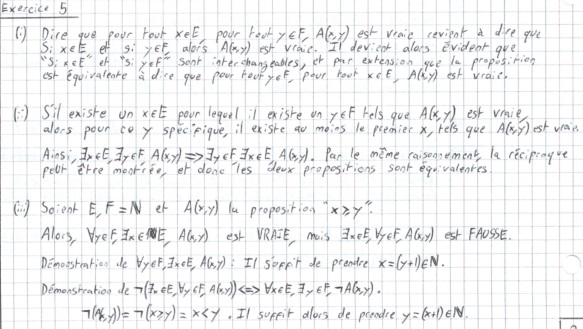
\includegraphics{ex05.jpg}
	
	\vspace{5mm}
	\noindent
	\textbf{Exercice 6.} (Fonctions caractéristiques $\chi_A$).
	Soient $E$ un ensemble et $A \subset E$. La fonction
	caractéristique de A est définie par $\chi_A : E \to \{0, 1\}$ et
	\[
		\chi_A : x \mapsto \left\{
		\begin{aligned}
			&1 & &\text{si}\ x \in A\\
			&0 & &\text{sinon.}
		\end{aligned}
		\right.
	\]
	
	\begin{enumerate}[label=(\roman*)]
		\item Montrer que deux ensembles sont égaux si et seulement
		si ils ont la même fonction caractéristique.
		
		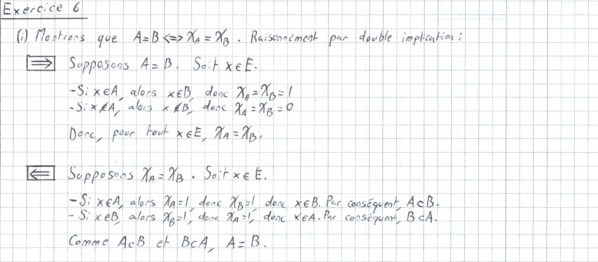
\includegraphics{ex06-1.jpg}
		%
		\newpage
		%
		\item Que peut-on dire sur $A$ et $B$ si
		$\chi_A(x) \leq \chi_B(x)$ pour tout $x \in E$ ?
		
		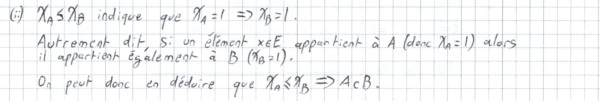
\includegraphics{ex06-2.jpg}
		%
		\item Montrer que $\chi_{A \cap B} = \chi_A \chi_B$,
		$\chi_{A^C} = 1 - \chi_A$ et
		$\chi_{A \cup B} = \chi_A + \chi_B - \chi_A \chi_B$.
		
		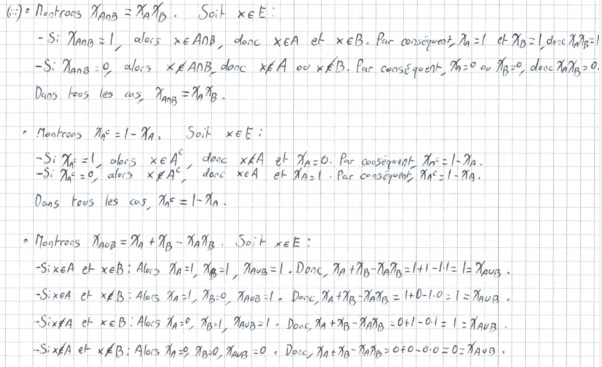
\includegraphics{ex06-3.jpg}
		%
		\item Montrer que les formules de De Morgan pour $(A \cup B)^C$
		et $(A \cap B)^C$ en utilisant les fonctions caractéristiques.
		
		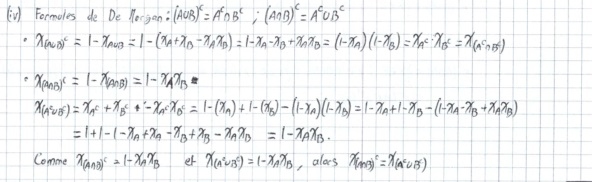
\includegraphics{ex06-4.jpg}
		%
	\end{enumerate}
	
	\newpage
	
	\noindent
	\textbf{Exercice 7.} Soit $f: E \to F$ une fonction bijective.
	Démontrer les propriétés suivantes énoncées mais pas démontrées
	en classe (Proposition 1.23).
	
	\begin{enumerate}[label=(\roman*)]
		\item $(f^{-1})^{-1} = f, \quad
			f^{-1} \circ f = I_E, \quad
			f \circ f^{-1} = I_F$.
		%
		\item (unicité de l'inverse) Si $g : F \to E$ tel que
		$g \circ f = I_E$ et $f \circ g = I_F$, alors $g = f^{-1}$.
		%
		\item (composition des inverses) Soit $g : F \to G$ une autre
		fonction bijective. Alors
		$(g \circ f)^{-1} = f^{-1} \circ g^{-1}$.
	\end{enumerate}
		
	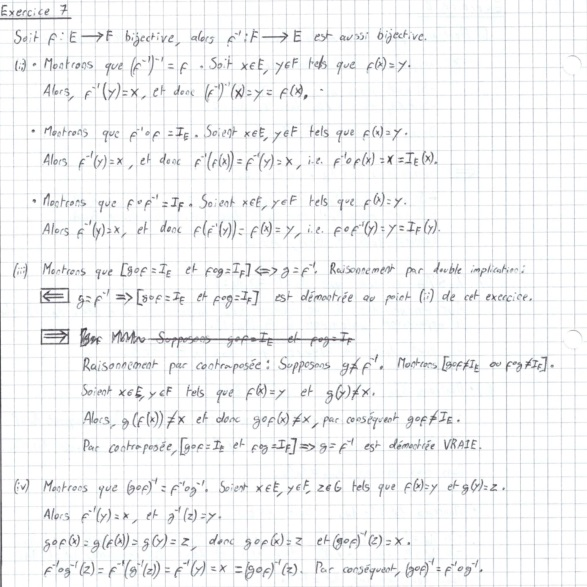
\includegraphics{ex07.jpg}
	
	\newpage
	\noindent
	\textbf{Exercice 8.} Soit $f : E \to F$ une fonction.
	
	\begin{enumerate}[label=(\roman*)]
		\item Soit $B \subset F$. Dans le cas où $f$ est bijective,
		montrer que l'image réciproque $f^{-1}(B)$ de $B$ est égale
		à l'image directe de $B$ par la fonction inverse $f^{-1}$.
		(Notons que l'image réciproque existe pour tout $f$, tandis
		que la fonction inverse uniquement si $f$ est bijective.)
		
		\colorbox{solution}
		{
			\begin{minipage}{0.9\textwidth}
				Soit $A \subset E$ tel que $B$ est l'image directe de
				$A$ par $f$, \textit{i.e.} $f(A) = B$. Alors l'image
				réciproque de $B$ est $f^{-1}(B) = A$.
				
				Comme $B$ est l'image directe de $A$, pour tout
				$y \in B$ il existe $x \in A$ tel que $f(x) = y$.
				Puisque $f$ est bijective, $x$ est unique et
				$f^{-1}(y) = x$. Donc $A$ est également l'image
				directe de $B$ par $f^{-1}$.
			\end{minipage}
		}
		%
		\item Montrer que pour tout $A, B \subset F$ on a
		\[
			f^{-1}(A \cup B) = f^{-1}(A) \cup f^{-1}(B), \quad
			f^{-1}(A \cap B) = f^{-1}(A) \cap f^{-1}(B)
		\]
		
		\colorbox{solution}
		{
			\begin{minipage}{0.9\textwidth}
				\[ \begin{split}
					f^{-1}(A \cup B) &= \{x \in E : f(x) \in A \cup B\}
					= \{x \in E : f(x) \in A \ \text{ou}\ f(x) \in B\}\\
					&= \{x \in E : f(x) \in A\}
						\cup \{x \in E : f(x) \in B\}
					= f^{-1}(A) \cup f^{-1}(B)
				\end{split}\]
				
				\[ \begin{split}
					f^{-1}(A \cap B) &= \{x \in E : f(x) \in A \cup B\}
					= \{x \in E : f(x) \in A \ \text{et}\ f(x) \in B\}\\
					&= \{x \in E : f(x) \in A\}
					\cap \{x \in E : f(x) \in B\}
					= f^{-1}(A) \cap f^{-1}(B)
				\end{split}\]
			\end{minipage}
		}
		%
		\item Montrer que pour tout $A, B \subset F$ on a
		\[
		f(A \cup B) = f(A) \cup f(B), \quad
		f(A \cap B) \subset f(A) \cap f(B)
		\]
		
		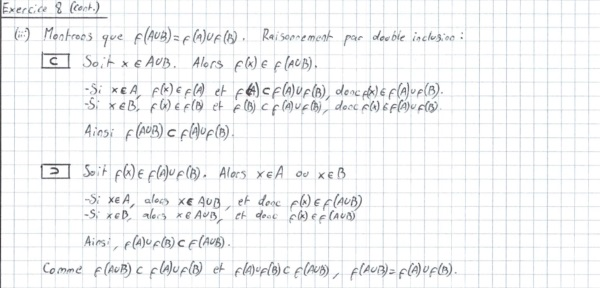
\includegraphics{ex08-3.jpg}
		%
		\item Montrer qu'en général $f(A \cap B) = f(A) \cap f(B)$
		est fausse.\\
		Montrer aussi qu'elle est vraie si $f$ est injective.
		
		\colorbox{solution}
		{
			\begin{minipage}{0.9\textwidth}
				Contre-exemple : $f: \mathbb{R} \to \mathbb{R},
					x \mapsto x^2$ avec 
				$A = \mathbb{R}_+$ et $B = \mathbb{R}_-$.\\				
				Alors $A \cap B = \{0\}$, et $f(A \cap B) = \{0\}$.
				Par contre, $f(A) = f(B) = f(A) \cap f(B)	
					= \mathbb{R}_+$.\\
					
				En revanche, si $f$ est injective :
				Soit $f(x) \in f(A) \cap f(B)$. Alors $f(x) \in f(A)$
				et $f(x) \in f(B)$, et comme $f$ est injective alors
				$x \in A$ et $x \in B$. Donc, $x \in A \cap B$ et
				$f(x) \in f(A \cap B)$.
				
				Par conséquent, $f(A) \cap f(B) \subset f(A \cap B)$
				et comme $f(A) \cap f(B) \supset f(A \cap B)$
				(démontrée au point (iii)), alors
				$f(A \cap B) = f(A) \cap f(B)$.
			\end{minipage}
		}
	\end{enumerate}
	
	\newpage
		
	\noindent
	\textbf{Exercice 9.}
	
	\begin{enumerate}[label=(\roman*)]
		\item Soit $E = \mathbb{R}^{\mathbb{Z}}$. Les éléments de $E$
		sont des familles $x = (x_i)_{i \in \mathbb{Z}}$ indexées par
		$\mathbb{Z}$. Définissons la fonction $f : E \to E$ par
		\[
		f : (x_i)_{i \in \mathbb{Z}} \mapsto (x_{i+1})_{i \in \mathbb{Z}}
		\]
		Montrer que $f$ est bijective et déterminer $f^{-1}$.
		%
		\item Soit $E = \mathbb{R}^{\mathbb{N}}$. Les éléments de $E$
		sont des familles $x = (x_i)_{i \in \mathbb{N}}$ indexées par
		$\mathbb{N}$ (aussi appelées suites).
		Définissons la fonction $f : E \to E$ par
		\[
		f : (x_i)_{i \in \mathbb{N}} \mapsto (x_{i+1})_{i \in \mathbb{N}}
		\]
		Est-ce que $f$ est injective ? Surjective ?
		%
		\item Soit $f$ la fonction de (ii). Définissons les ensembles
		$A, B \subset \mathbb{R}^{\mathbb{N}}$ par
		\[
		A = \{(x_i)_{i \in \mathbb{N}} : x_0 \in [0,1], x_1 \leq 0\},
		\quad
		B = \{(x_i)_{i \in \mathbb{N}} : \exists i \in \mathbb{N}, x_i \geq 0\}
		\]
		Déterminer les images directes $f(A)$ et $f(B)$ ainsi que les
		images réciproques $f^{-1}(A)$ et $f^{-1}(B)$.
	\end{enumerate}
		
	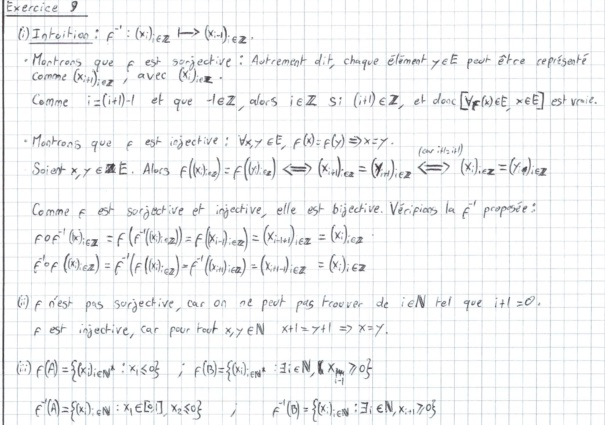
\includegraphics{ex09.jpg}
		
\end{document}
